\let\negmedspace\undefined
\let\negthickspace\undefined
\documentclass[journal]{IEEEtran}
\usepackage[a5paper, margin=10mm, onecolumn]{geometry}
%\usepackage{lmodern} % Ensure lmodern is loaded for pdflatex
\usepackage{tfrupee} % Include tfrupee package

\setlength{\headheight}{1cm} % Set the height of the header box
\setlength{\headsep}{0mm}     % Set the distance between the header box and the top of the text

\usepackage{gvv-book}
\usepackage{gvv}
\usepackage{cite}
\usepackage{amsmath,amssymb,amsfonts,amsthm}
\usepackage{algorithmic}
\usepackage{graphicx}
\usepackage{textcomp}
\usepackage{xcolor}
\usepackage{txfonts}
\usepackage{listings}
\usepackage{enumitem}
\usepackage{mathtools}
\usepackage{gensymb}
\usepackage{comment}
\usepackage[breaklinks=true]{hyperref}
\usepackage{tkz-euclide} 
\usepackage{listings}
% \usepackage{gvv}                                        
\def\inputGnumericTable{}                                 
\usepackage[latin1]{inputenc}                                
\usepackage{color}                                            
\usepackage{array}                                            
\usepackage{longtable}                                       
\usepackage{calc}                                             
\usepackage{multirow}                                         
\usepackage{hhline}                                           
\usepackage{ifthen}                                           
\usepackage{lscape}
\begin{document}

\bibliographystyle{IEEEtran}
\vspace{3cm}

\title{5.9.14}
\author{EE25BTECH11060 - V.Namaswi}
% \maketitle
% \newpage
% \bigskip
{\let\newpage\relax\maketitle}
\renewcommand{\thefigure}{\theenumi}
\renewcommand{\thetable}{\theenumi}
\setlength{\intextsep}{10pt} % Space between text and floats
\textbf{Question}\\ On her birthday Seema decided to donate some money to children of an orphanage home. If there were 8 children less, every one would have got  10 Rupees more. However,if there were 16 children more, every one would have got  10 Rupees less. Using matrix method, find the number of children and the amount distributed by Seema. What values are reflected by Seemas decision ?\\
\textbf{Solution}\\
Let, Number of children=c and Amount=a\\
Given,\\
\begin{align}
   ca=(c-8)(a+10)=(c+16)(a-10) 
\end{align}
From 1,
\begin{align}
    10c-8a=80\\
    10c-16a=-160
\end{align}
   From 2,
\begin{align}
    \begin{pmatrix}
        5 \\ -4
    \end{pmatrix}^\top \begin{pmatrix}
        c \\ a
    \end{pmatrix}=40
    \end{align}
    From 3,
\begin{align}
    \begin{pmatrix}
     5  \\ -8   
    \end{pmatrix}^\top \begin{pmatrix}
        c \\ a
    \end{pmatrix}=-80\\
    \begin{pmatrix}
        5 & -4 \\
        5 & -8
    \end{pmatrix}\begin{pmatrix}
        c \\ a
    \end{pmatrix}=\begin{pmatrix}
        40 \\ -80
    \end{pmatrix}
\end{align} 
 
   Forming argumented matrix
\begin{align}
    \augvec{2}{1}{5 & -4 & 40 \\ 5 & -8 & -80}
\end{align}
Replace
\[R_2 \to R_2-R_1\]
\begin{align}
\augvec{2}{1}{5 & -4 & 40 \\ 0 & -4 & -120} 
    \end{align}
Replace
\[R_2 \to R_2/-4\]
\begin{align}
      \augvec{2}{1}{5 & -4 & 40 \\ 0 & 1 & 30} 
\end{align}
 Replace
\[R_1 \to R_1+4R_2\]
\begin{align}
    \augvec{2}{1}{5 & 0 & 160 \\ 0 & 1 & 30} 
\end{align} 
Replace
\[R_1 \to R_1/5\]
\begin{align}
      \augvec{2}{1}{1 & 0 & 32 \\ 0 & 1 & 30} 
\end{align}
so,
\begin{align}
    c=32 \quad  a=30
\end{align}
Refer fig
\begin{align}
\centering
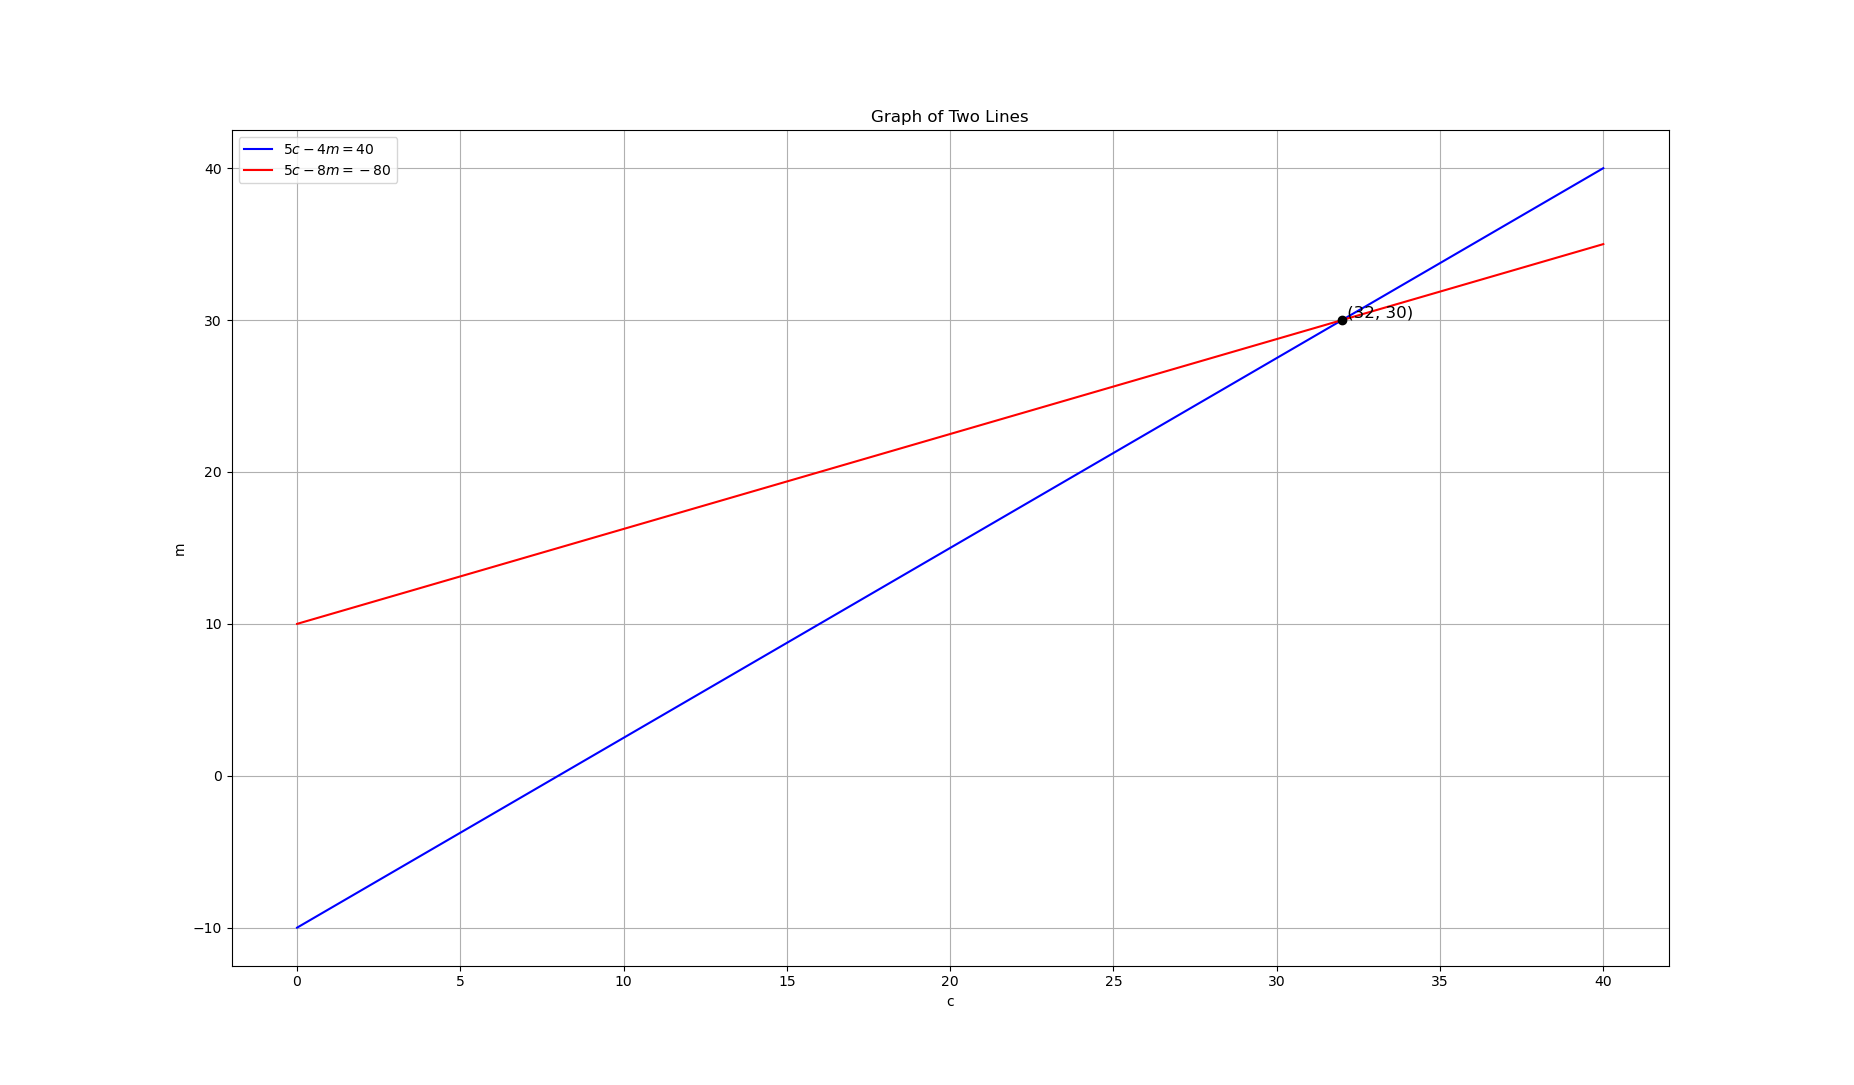
\includegraphics[width=\columnwidth, height=0.8\textheight, keepaspectratio]{figs/Figure_12 .png}   
\end{align}
\end{document}